\section{Frontend}
\rhead{Frontend}

A frontend a szoftver azon része, amely nagyban meghatározza egy felhasználó élményét. Fontos az átláthatóság, a könnyű kezelhetőség és az esztétika. Ezen szempontokat figyelembe véve készítettük el az Archytex weboldalt.

\subsection{Design terv}
A honlap elkészítésének első lépése a tervezés volt. Ehhez a Figma\footnote{\url{https://www.figma.com/}} nevű ingyenes design szoftvert használtuk. Ezen alkalmazás segítségével könnyedén tudtunk vázlatot készíteni arról, hogy hogyan képzeljük el a honlap megjelenését, még azelőtt, hogy elkezdtük volna a programozást.

A Figma a design tervezés mellett használható vektor grafikák rajzolására is, amellyel az Archytex szerkesztőben látható ikonok készültek.

\begin{figure}[h]
  \centering
  
\includegraphics[width=0.1\textwidth]{parts/developer-documentation/frontend/images/meshSelectMode.png}
  
\includegraphics[width=0.1\textwidth]{parts/developer-documentation/frontend/images/faceSelectMode.png}
  
\includegraphics[width=0.1\textwidth]{parts/developer-documentation/frontend/images/vertexSelectMode.png}
  \caption{Példa a Figma-ban készíthető vektor grafikákra: kiválasztási mód ikonjai az Archytex szerkesztőből.}
\end{figure}

% TODO: Undraw.io
Undraw.io

% TODO: Logo design paragraph + Logo image
Logo design


\subsection{Használt technológiák}
A frontend alkalmazás React-ben\footnote{\url{https://hu.reactjs.org/}} készült. Azért esett a választás erre a keretrendszerre, mert a horog alapú komponens állapot- és és életcikluskezelése miatt fejlesztői élményét tekintve kiemelkedően jobb, mint más rendszerek. Emellett az is segítette a választást, hogy jelenleg a React a legnépszerűbb a webfejlesztők köreiben\cite{most-used-web-frameworks}, ezért rengeteg forrás és oktatóvideó érhető el hozzá.

A honlap elkészítéséhez a Material UI\footnote{\url{https://mui.com/}} nevű komponens könyvtárat használtuk, amely rengeteg előre elkészített és könnyen testreszabható komponenst tartalmaz. Ennek segítségével és a Google által kifejlesztett Material Design\footnote{\url{https://material.io/}} irányelveit követve modern, letisztult és felhasználóbarát felületet tudtunk létrehozni.

\subsection{Főoldal}
A főoldal célja, hogy egy új felhasználónak "eladja" a termékünket. Ezért fontos volt, hogy látványos és emlékezetes legyen, de ezek mellett egyben informatív is. A látványossághoz nagyban hozzájárultak az Undraw.io-s illusztrációk és a tsparticles\footnote{\url{https://github.com/matteobruni/tsparticles/tree/main/components/react}} JavaScript könyvtár segítségével létrehozott, az oldal fejlécében megjelenő interaktív buborékok. Emellett az interaktívitás növelése érdekében az AOS (Animate On Scroll) könyvtárat használva megoldottuk, hogy a honlap tartalma folyamatosan jelenjen meg, ahogy a felhasználó görget lefelé a honlapon.

\begin{figure}[h]
  \centering
  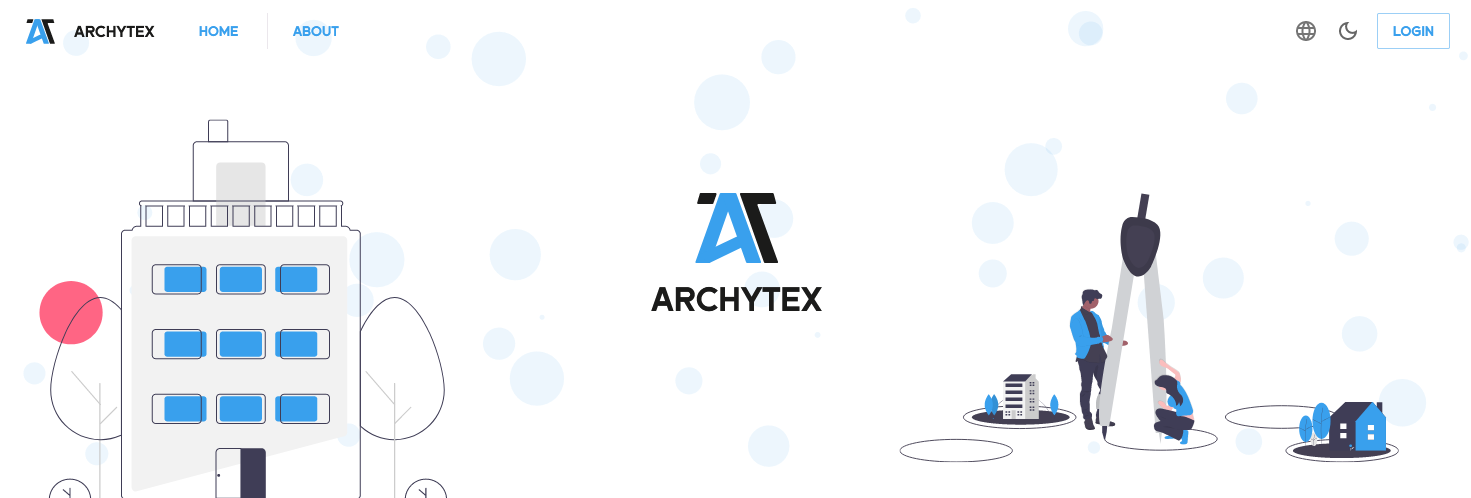
\includegraphics[width=\textwidth]{parts/developer-documentation/frontend/images/header.png}
  \caption{Az Archytex főoldal fejléce}
\end{figure}

\subsection{Autentikáció}
A bejelentkezési és regisztrációs képernyő funkcionalitás szempontjából egy viszonylag nagyobb kihívást nyújtott, mint más oldalak. Tudtuk, hogy gyakran lesz szükségünk olyan űrlapokra a projekt folyamán, amiben a felhasználó felé visszajelzést kell küldeni, ezért készítettünk egy generalizált React komponenst ennek a feladatnak az ellátására.

\subsection{Irányítópult}

\subsection{Editor}

\subsection{Tesztek}